% Creating a simple Title Page in Beamer
\documentclass[spanish]{beamer}
\usepackage[spanish]{babel}
\usepackage{tikz}
\usepackage{graphicx}
\usepackage{tcolorbox}
\usetikzlibrary{er,positioning}

% Theme choice:
\usetheme{AnnArbor}

% Title page details: 
\title{Diseño de una base de datos}
\author{Alexis Ovalle}
\date{\today}

\begin{document}

% Title page frame
\begin{frame}
    \titlepage
\end{frame}

\begin{frame}
\frametitle{Indice}
\tableofcontents
\end{frame}


\section{Estructura relacional}
  % ======= ENTIDAD =======
\begin{frame}{Entidad}
    \begin{tcolorbox}[title=Entidad,colback=blue!5!white,colframe=blue!75!black]
        Una entidad es un objeto del mundo real que puede distinguirse de otros objetos y sobre el cual se almacena información en una base de datos. 
        Puede representar una persona, lugar, evento o cosa de interés. 
        \textbf{Ejemplo:} Un cliente en un sistema de ventas.
    \end{tcolorbox}
\end{frame}

% ======= ATRIBUTO =======
\begin{frame}{Atributo}
    \begin{tcolorbox}[title=Atributo,colback=green!5!white,colframe=green!75!black]
        Un atributo es una característica o propiedad de una entidad. 
        Los atributos pueden ser simples o compuestos, monovalorados o multivalorados.
        \textbf{Ejemplo:} El nombre y la dirección de un Cliente.
    \end{tcolorbox}
\end{frame}

% ======= REGISTRO =======
\begin{frame}{Registro}
    \begin{tcolorbox}[title=Registro,colback=yellow!5!white,colframe=yellow!75!black]
        Un registro es una fila en una tabla de base de datos que representa una instancia específica de una entidad. 
        Cada registro está compuesto por un conjunto de valores de atributos.
        \textbf{Ejemplo:} Un registro en la tabla clientes con los datos de Juan Pérez.
    \end{tcolorbox}
\end{frame}
% ======= CLAVE =======
\begin{frame}{Clave}
    \begin{tcolorbox}[title=Clave,colback=cyan!5!white,colframe=cyan!75!black]
        Una clave es un conjunto de uno o más atributos que identifican de manera única un registro dentro de una tabla en la base de datos.
        
        \textbf{Tipos de Claves:}
        \begin{itemize}
            \item \textbf{Clave primaria (Primary Key):} Identifica de forma única cada registro en una tabla.
            \item \textbf{Clave candidata (Candidate Key):} Conjunto mínimo de atributos que pueden ser clave primaria.
            \item \textbf{Clave foránea (Foreign Key):} Relaciona dos tablas asegurando la integridad referencial.
            \item \textbf{Clave compuesta (Composite Key):} Clave formada por dos o más atributos.
        \end{itemize}
   
    \end{tcolorbox}
\end{frame}

% ======= EJEMPLOS DE CLAVES =======
\begin{frame}{Ejemplos de Claves}
    \begin{tcolorbox}[title=Ejemplos de Claves,colback=gray!5!white,colframe=gray!75!black]
        \textbf{Ejemplo 1: Clave Primaria}  
        En la tabla \texttt{Clientes}, el \texttt{ID\_Cliente} es la clave primaria porque identifica de manera única a cada cliente.  

        \begin{table}[]
            \centering
            \begin{tabular}{|c|c|c|}
                \hline
                \textbf{ID\_Cliente} & \textbf{Nombre}  & \textbf{Correo}          \\
                \hline
                1           & Juan Pérez  & juan@email.com    \\
                2           & María López & maria@email.com   \\
                3           & Pedro Gómez & pedro@email.com   \\
                \hline
            \end{tabular}
            \caption{Ejemplo de Clave Primaria}
        \end{table}

    \end{tcolorbox}
\end{frame}

\begin{frame}{Ejemplos de Claves}
    \begin{tcolorbox}[title=Ejemplos de Claves,colback=gray!5!white,colframe=gray!75!black]
        \textbf{Ejemplo 2: Clave Foránea}  
        En la tabla \texttt{Pedidos}, el \texttt{ID\_Cliente} es una clave foránea que referencia a la tabla \texttt{Clientes}, garantizando la integridad de los datos.

        \begin{table}[]
            \centering
            \begin{tabular}{|c|c|c|}
                \hline
                \textbf{ID\_Pedido} & \textbf{ID\_Cliente} & \textbf{Total} \\
                \hline
                101         & 1             & Q250.00  \\
                102         & 2             & Q300.00  \\
                103         & 1             & Q150.00  \\
                \hline
            \end{tabular}
            \caption{Ejemplo de Clave Foránea}
        \end{table}
    \end{tcolorbox}
\end{frame}

% ======= EJEMPLOS DE CLAVE COMPUESTA Y CANDIDATA =======
\begin{frame}{Ejemplos de Claves}
    \begin{tcolorbox}[title=Ejemplos de Claves,colback=gray!5!white,colframe=gray!75!black]
        
        \textbf{Ejemplo 3: Clave Compuesta}  
         Una clave compuesta se forma utilizando dos o más atributos para identificar de manera única una fila en la tabla.  
        
        En la tabla \texttt{Ingreso\_Productos}, la combinación de \texttt{ID\_Producto} y \texttt{Fecha\_Ingreso} forman la clave primaria porque juntos identifican de manera única cada ingreso de producto en el inventario.


        \begin{table}[]
            \centering
            \resizebox{0.80\textwidth}{!}{
       \begin{tabular}{|c|c|c|c|}
                \hline
                \textbf{ID\_Producto} & \textbf{Fecha\_Ingreso} & \textbf{Cantidad} & \textbf{Proveedor} \\
                \hline
                10         & 2024-02-15       & 50         & Empresa A  \\
                15         & 2024-02-16       & 30         & Empresa B  \\
                10         & 2024-02-17       & 20         & Empresa C  \\
                \hline
            \end{tabular}
            }

            \caption{Ejemplo de Clave Compuesta}
        \end{table}

 
    \end{tcolorbox}
\end{frame}

% ======= EJEMPLOS DE CLAVE COMPUESTA Y CANDIDATA =======
\begin{frame}{Ejemplos de Claves}
    \begin{tcolorbox}[title=Ejemplos de Claves,colback=gray!5!white,colframe=gray!75!black]
        

        \textbf{Ejemplo 4: Clave Candidata}  
        Una clave candidata es un conjunto de atributos que pueden ser claves primarias, pero solo se elige una.  

        En la tabla \texttt{Usuarios}, tanto el \texttt{ID\_Usuario} como el \texttt{Correo} son claves candidatas porque ambos identifican de manera única a un usuario. Sin embargo, solo una se usa como clave primaria.

        \begin{table}[]
            \centering
            \begin{tabular}{|c|c|c|}
                \hline
                \textbf{ID\_Usuario} & \textbf{Correo} & \textbf{Nombre}  \\
                \hline
                1           & juan@email.com    & Juan Pérez  \\
                2           & maria@email.com   & María López \\
                3           & pedro@email.com   & Pedro Gómez \\
                \hline
            \end{tabular}
            \caption{Ejemplo de Clave Candidata}
        \end{table}
    \end{tcolorbox}
\end{frame}

% ======= RELACIÓN =======
\begin{frame}{Relación}
    \begin{tcolorbox}[title=Relación,colback=red!5!white,colframe=red!75!black]
        Una relación representa la asociación entre dos o más entidades en una base de datos. 
        Puede ser de diferentes tipos: uno a uno (1:1), uno a muchos (1:N) o muchos a muchos (M:N).
        \textbf{Ejemplo:} La relación compra entre clientes y productos.
    \end{tcolorbox}
\end{frame}

% ======= ENTIDAD DÉBIL =======
\begin{frame}{Entidad Débil}
    \begin{tcolorbox}[title=Entidad Débil,colback=purple!5!white,colframe=purple!75!black]
        Una entidad débil es aquella que no tiene un identificador propio y depende de una entidad fuerte para su existencia. 
        Se identifica mediante una clave foránea.
        \textbf{Ejemplo:} Historial Médico en relación con Paciente.
    \end{tcolorbox}
\end{frame}

% ======= DOMINIO =======
\begin{frame}{Dominio}
    \begin{tcolorbox}[title=Dominio,colback=gray!5!white,colframe=gray!75!black]
        Un dominio es el conjunto de valores permitidos para un atributo en una base de datos. 
        Define restricciones sobre los valores que pueden ser almacenados en un campo específico.
        \textbf{Ejemplo:} El dominio del atributo edad puede ser un rango de 0 a 120 años.
    \end{tcolorbox}
\end{frame}


% ======= SQL: Lenguaje de Consulta Estructurado y Categorías =======
\begin{frame}{SQL: Lenguaje de Consulta Estructurado y Categorías}
    \begin{tcolorbox}[title=SQL,colback=orange!5!white,colframe=orange!75!black]
        
        \textbf{¿Qué es SQL?}  
        SQL (Structured Query Language) es un lenguaje estándar utilizado para gestionar y manipular bases de datos.  
        Permite interactuar con las bases de datos mediante la ejecución de diversas consultas y operaciones.

        \textbf{Categorías de SQL:}  
        SQL se clasifica en varias categorías, las cuales definen el tipo de operaciones que se pueden realizar:

        \begin{itemize}
            \item \textbf{DDL (Data Definition Language):}  
                Se utiliza para definir, modificar y eliminar estructuras de base de datos, como tablas, índices y esquemas.  
                \begin{itemize}
                    \item \texttt{CREATE TABLE} - Crea una nueva tabla.
                    \item \texttt{ALTER TABLE} - Modifica la estructura de una tabla existente.
                    \item \texttt{DROP TABLE} - Elimina una tabla.
                \end{itemize}


        \end{itemize}
    \end{tcolorbox}
\end{frame}
% ======= SQL: Lenguaje de Consulta Estructurado y Categorías =======
\begin{frame}{SQL: Lenguaje de Consulta Estructurado y Categorías}
    \begin{tcolorbox}[title=SQL,colback=orange!5!white,colframe=orange!75!black]
        \textbf{Categorías de SQL:}  
        \begin{itemize}
            \item \textbf{DML (Data Manipulation Language):}  
                Permite manipular los datos dentro de las tablas.  
                \begin{itemize}
                    \item \texttt{SELECT} - Consulta los datos de una tabla.
                    \item \texttt{INSERT} - Inserta nuevos datos en una tabla.
                    \item \texttt{UPDATE} - Modifica datos existentes en una tabla.
                    \item \texttt{DELETE} - Elimina datos de una tabla.
                \end{itemize}

            \item \textbf{DCL (Data Control Language):}  
                Se utiliza para controlar el acceso a los datos y gestionar los permisos de los usuarios.  
                \begin{itemize}
                    \item \texttt{GRANT} - Asigna permisos a un usuario.
                    \item \texttt{REVOKE} - Revoca permisos a un usuario.
                \end{itemize}


              
      
        \end{itemize}
    \end{tcolorbox}
\end{frame}


% ======= SQL: Lenguaje de Consulta Estructurado y Categorías =======
\begin{frame}{SQL: Lenguaje de Consulta Estructurado y Categorías}
    \begin{tcolorbox}[title=SQL,colback=orange!5!white,colframe=orange!75!black]
        \textbf{Categorías de SQL:}  
        \begin{itemize}


            \item \textbf{TCL (Transaction Control Language):}  
                Se usa para gestionar las transacciones en las bases de datos.  
              
                \begin{itemize}
                    \item \texttt{COMMIT} - Confirma una transacción.
                    \item \texttt{ROLLBACK} - Revierte una transacción.
                    \item \texttt{SAVEPOINT} - Establece un punto de guardado dentro de una transacción.
                \end{itemize}
        \end{itemize}
    \end{tcolorbox}
\end{frame}


\begin{frame}{Modelo conceptual, lógico y físico}
    \begin{itemize}
        \item \textbf{Modelo conceptual}: Descripción abstracta del sistema, sin detalles sobre su implementación.
        \item \textbf{Modelo lógico}: Representación más detallada, con un enfoque en las relaciones entre los elementos del sistema.
        \item \textbf{Modelo físico}: Implementación concreta del sistema, considerando aspectos de hardware, software y tecnología.
    \end{itemize}
\end{frame}



%%%%%%%%%%%%%%%%%%%% INICIO SECCION 2
%%%%%%%%%%%%%%%%%%%% %%%%%%%%%%%%%%%%%%%% %%%%%%%%%%%%%%%%%%%%
%%%%%%%%%%%%%%%%%%%% %%%%%%%%%%%%%%%%%%%% %%%%%%%%%%%%%%%%%%%%
%%%%%%%%%%%%%%%%%%%% %%%%%%%%%%%%%%%%%%%% %%%%%%%%%%%%%%%%%%%%
%%%%%%%%%%%%%%%%%%%% %%%%%%%%%%%%%%%%%%%% %%%%%%%%%%%%%%%%%%%%
%%%%%%%%%%%%%%%%%%%% %%%%%%%%%%%%%%%%%%%% %%%%%%%%%%%%%%%%%%%%
\section{Ejemplo}
    \begin{frame}{Descripción}
    El sistema RENAP (Registro Nacional de las Personas) gestiona y automatiza los procesos de registro civil y emisión de documentos oficiales, facilitando el acceso a la información clave de los ciudadanos.
    \textbf{Elementos a considerar}
    \begin{itemize}
        \item Registro de nacimientos
        \item Registro de defunciones
        \item Registro de matrimonios
        \item Registro de divorcios
        \item Generar DPI 
        \item Certificacion documentos
        \item Obtener documentos
        \item Tarifario
        
    \end{itemize}
    \end{frame}
    \begin{frame}{¿Con que contamos?}
        \textbf{Análisis del sistema}
        En primera instancia el RENAP es el registro de personas, así que \textbf{persona} sera algo fundamental.
        \\
        \textbf{Que elementos tiene una persona?}
\begin{table}[h]
    \centering
    \resizebox{0.90\textwidth}{!}{ % Escala la tabla al 75% del ancho
        \begin{tabular}{|c|l|c|l|l|l|c|l|}
            \hline
            ID & Nombre Completo & Fecha de nacimiento & Lugar Nacimiento & Lugar Residencia & País & Sexo & Estado Civil \\
            \hline
            1  & Juan Pérez  & 25/02/2005  & Guatemala  & Quetzaltenango & Guatemala & M & Soltero \\
            2  & María Gómez  & 30/09/1985  & Guatemala  & Ciudad de Guatemala & Guatemala & F & Casada \\
            3  & Pedro López  & 28/11/1999  & El Salvador & San Salvador & El Salvador & M & Soltero \\
            \hline
        \end{tabular}
    }
    \caption{Ejemplo de persona}
    \label{tab:ejemplo}
\end{table}

    \end{frame}

    \begin{frame}{Diagrama}
        \begin{center}
        \begin{tikzpicture}[scale=0.8, transform shape] % Reduce tamaño global
            \node[entity] (Persona) {Persona};
            \node[attribute, left=1.5cm of Persona] (ID) {\tiny ID} edge (Persona);
            \node[attribute, above left=0.8cm and 1.5cm of Persona] (Nombre) {\tiny Nombre} edge (Persona);
            \node[attribute, above right=0.8cm and 1.5cm of Persona] (Edad) {\tiny Edad} edge (Persona);
            \node[attribute, below left=0.8cm and 1.5cm of Persona] (LugarNac) {\tiny Nacimiento} edge (Persona);
            \node[attribute, below right=0.8cm and 1.5cm of Persona] (LugarRes) {\tiny Residencia} edge (Persona);
            \node[attribute, right=1.5cm of Persona] (Pais) {\tiny País} edge (Persona);
            \node[attribute, below=1.5cm of Persona] (Sexo) {\tiny Sexo} edge (Persona);
            \node[attribute, below right=1.5cm and 1.5cm of Persona] (Estado) {\tiny Estado} edge (Persona);
        \end{tikzpicture}
        \end{center}


    \end{frame}
    \begin{frame}{¿Qué defino por acta de nacimiento?}
           \begin{figure}
                \centering
                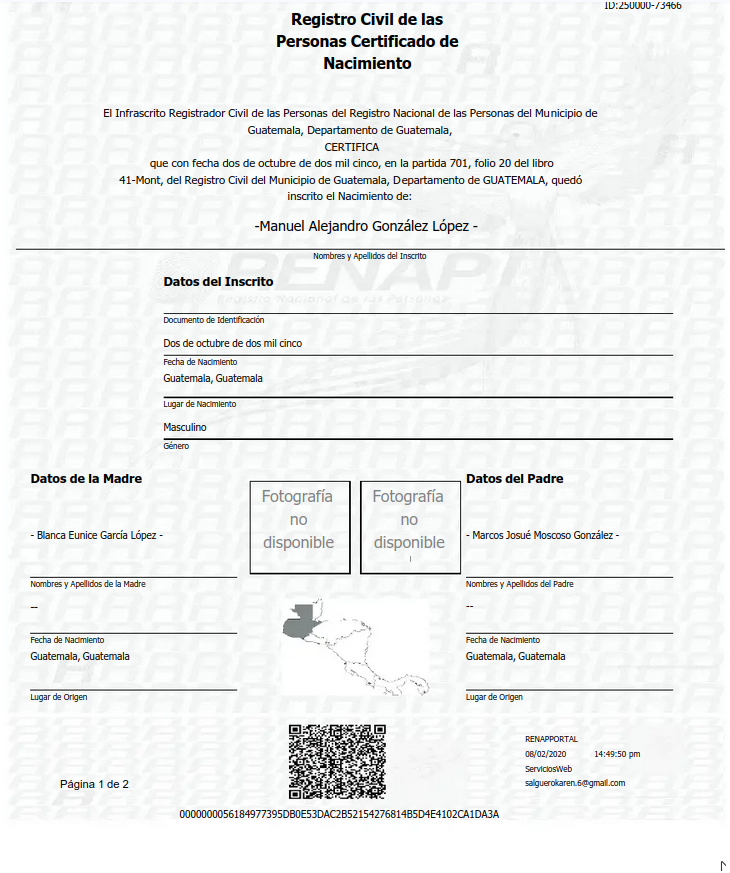
\includegraphics[width=0.6\textwidth]{img/nacimiento.png}
                \caption{Diagrama de las categorías de SQL}
            \end{figure}
    \end{frame}
        \begin{frame}{¿Qué defino por acta de nacimiento?}
\begin{table}[h]
    \centering
    \resizebox{0.90\textwidth}{!}{ % Escala la tabla al 90% del ancho
        \begin{tabular}{|c|l|c|c|c|}
            \hline
            ID & Nombre Completo & DPI Persona & DPI Padre 1 & DPI Padre 2 \\
            \hline
            1  & Juan Pérez  & 1234567890123  & 9876543210123 & 1122334455667 \\
            2  & María Gómez  & 2345678901234  & 2233445566778 & 9988776655443 \\
            3  & Luis Hernández  & 3456789012345  & 5566778899001 & 6677889900112 \\
            \hline
        \end{tabular}
    }
    \caption{Ejemplo de Acta de Nacimiento}
    \label{tab:acta_nacimiento}
\end{table}

    \end{frame}
      \begin{frame}{¿Qué defino por acta de defunción?}
                \begin{figure}
                \centering
                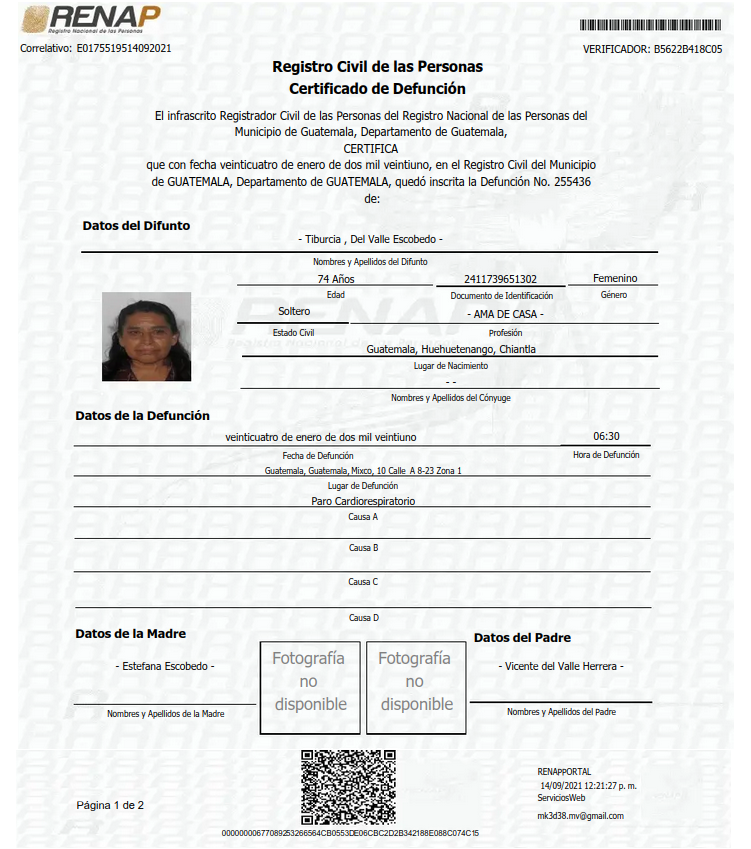
\includegraphics[width=0.6\textwidth]{img/defuncion.png}
                \caption{Diagrama de las categorías de SQL}
            \end{figure}
    \end{frame}
    
    \begin{frame}{¿Qué defino por acta de defunción?}
        \begin{table}[h]
            \centering
            \resizebox{0.90\textwidth}{!}{ % Escala la tabla al 90% del ancho
                \begin{tabular}{|c|l|c|c|l|l|}
                    \hline
                    ID & Nombre Completo & Fecha de Defunción & Hora de Defunción & Lugar de Defunción & Causas de Muerte \\
                    \hline
                    1  & Juan Pérez  & 25/02/2023  & 14:30  & Quetzaltenango, Guatemala  & Enfermedad Cardíaca \\
                    2  & María Gómez  & 30/09/2022  & 08:00  & Ciudad de Guatemala, Guatemala  & Accidente de Tráfico \\
                    3  & Pedro López  & 15/11/2021  & 22:15  & Chimaltenango, Guatemala  & Cáncer Pulmonar \\
                    \hline
                \end{tabular}
            }
            \caption{Ejemplo de Acta de Defunción (Guatemala)}
            \label{tab:acta_defuncion}
        \end{table}
        
    \end{frame}
      \begin{frame}{¿Qué defino por acta de matrimonio?}
                   \begin{figure}
                        \centering
                        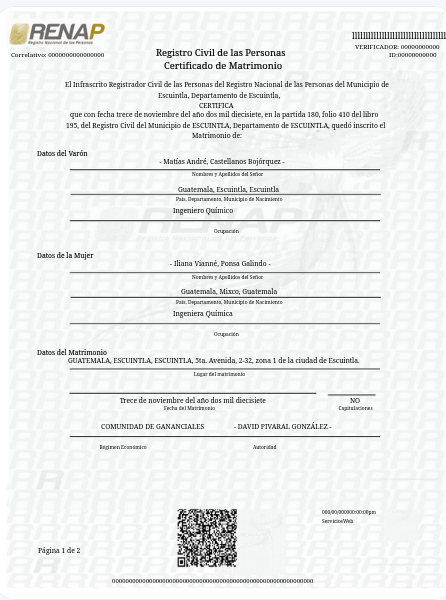
\includegraphics[width=0.6\textwidth]{img/matrimonio.png}
                        \caption{Diagrama de las categorías de SQL}
                    \end{figure}
    \end{frame}

    \begin{frame}{¿Qué defino por acta de matrimonio?}
    El registro, avisos de matrimonio se dejan en RENAP y se inscribe gratis
        \begin{table}[h]
            \centering
            \resizebox{0.90\textwidth}{!}{ % Escala la tabla al 90% del ancho
                \begin{tabular}{|c|l|l|l|l|l|c|}
                    \hline
                    ID & Persona 1 & Persona 2 & Lugar de Matrimonio & Capitulaciones & Régimen Económico & ID Autoridad \\
                    \hline
                    1  & Juan Pérez  & María Gómez  & Iglesia de la Merced, Ciudad de Guatemala  & Sin Capitulaciones  & Sociedad Conyugal  & 1234 \\
                    2  & Pedro López  & Ana Sánchez  & Registro Civil, Quetzaltenango  & Con Capitulaciones  & Separación de Bienes  & 5678 \\
                    3  & Luis Hernández  & Sofía Martínez  & Parroquia San Juan, Escuintla  & Con Capitulaciones  & Sociedad Conyugal  & 9101 \\
                    \hline
                \end{tabular}
            }
            \caption{Ejemplo de Acta de Matrimonio (Guatemala)}
            \label{tab:acta_matrimonio}
        \end{table}
    \end{frame}
      \begin{frame}{¿Qué defino por acta de divorcio?}
          \begin{table}[h]
            \centering
            \resizebox{0.90\textwidth}{!}{ % Escala la tabla al 90% del ancho
                \begin{tabular}{|c|l|c|c|c|}
                    \hline
                    ID & Acta Matrimonio ID & Fecha de Separación & ID Autoridad & Motivo de Divorcio \\
                    \hline
                    1  & 1234  & 10/01/2023  & 5678  & Incompatibilidad de Caracteres \\
                    2  & 5678  & 20/06/2022  & 9101  & Violencia Familiar \\
                    3  & 9101  & 05/03/2021  & 1122  & Abandono de Hogar \\
                    \hline
                \end{tabular}
            }
            \caption{Ejemplo de Acta de Divorcio (Guatemala)}
            \label{tab:acta_divorcio}
        \end{table}
        
    \end{frame}

      \begin{frame}{¿Qué defino por tarifario?}
        \begin{table}[h]
            \centering
            \resizebox{0.90\textwidth}{!}{ % Escala la tabla al 90% del ancho
                \begin{tabular}{|c|l|c|}
                    \hline
                    ID & Trámite & Precio (GTQ) \\
                    \hline
                    1  & Acta de Nacimiento  & 15 \\
                    2  & DPI  & 100 \\
                    3  & Matrimonio  & 25 \\
                    4  & Defunción  & 25 \\
                    \hline
                \end{tabular}
            }
            \caption{Tarifario de Trámites (Guatemala)}
            \label{tab:tarifario_tramites}
        \end{table}

        
    \end{frame}


    
      \begin{frame}{¿Qué defino por obtencion de documentos?}

        \begin{table}[h]
            \centering
            \resizebox{0.90\textwidth}{!}{ % Escala la tabla al 90% del ancho
                \begin{tabular}{|c|c|c|c|l|l|l|l|}
                    \hline
                    ID Documento & ID Persona & Cantidad a Pagar (GTQ) & Fecha de Pago & Lugar de Pago & A Domicilio & Recargo (GTQ) & Ubicación \\
                    \hline
                    1  & 123456  & 15  & 12/02/2023  & Virtual  & No  & 0  & - \\
                    2  & 234567  & 100 & 15/02/2023  & Presencial  & No  & 0  & - \\
                    3  & 345678  & 26  & 18/02/2023  & Virtual  & Sí  & 20  & Quetzaltenango \\
                    4  & 456789  & 15  & 20/02/2023  & Presencial  & Sí  & 15  & Ciudad de Guatemala \\
                    \hline
                \end{tabular}
            }
            \caption{Registro de Obtención de Documentos (Guatemala) con Opciones a Domicilio}
            \label{tab:registro_documentos_domicilio}
        \end{table}

        
    \end{frame}

\end{document}